\section{Discussion}

% Relation to previous work / Should rewrite this paragraph!
In our previous study, we demonstrated that oculomotor signals play a substantial role in the perception of self-motion, even in the absence of optic flow or any other visual stimulation \cite{clemens2015a}. Although the vestibular system provided the most significant contribution, oculomotor signals were shown to account for about 20\% of the overall percept. Because these experiments were performed with a single fixation depth, it was not clear whether the brain weighted the oculomotor signal in a depth-dependent manner when using it as a translation cue, or merely uses the signal as a rudimentary cue to self-motion. In the present study we tested between these two possibilities.

% Basic observations
We assessed self-motion perception during either body- and world-centered fixation at two different fixation depths. Our results show that self-motion was underestimated when comparing far and near fixation trials in the world-centered condition, which argues against a proper scaling of the eye movement signal. Fixation depth did not influence self-motion perception during body-centered fixation (where eye movements are virtually absent).  

% Model results
To quantify the relative depth-dependent scaling of eye movements for nearby and far away fixation targets, we fitted a straightforward linear model to the perceptual responses based on the oculomotor behavior across four conditions. While two participants show partial scaling, the other six participants did not show any sign of scaling. Thus, we conclude that while oculomotor signals provide a robust clue to translation perception, they are not properly scaled by fixation depth.


\subsection{Relation to other studies}

% Relation to Clemens, 2015
\begin{figure}
    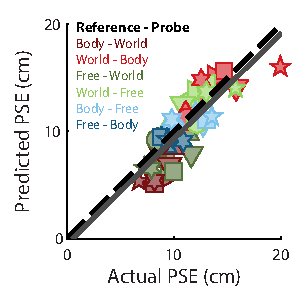
\includegraphics[width=0.5\textwidth]{src/paper4/p4_figure6.pdf}

    \caption{...}
    \label{p4:fig6}
\end{figure}

In our previous experiment we compared body-fixed to world-fixed fixations at near (50 \si{\centi\metre}) distances only \cite{clemens2015a}. We compared the parameter, $\alpha$, found in that paper with the parameters for the near condition, $\alpha_{50}$, found in the present study. \figref{p4:fig6} shows how well our $\alpha_{50}$ parameter explains the data in our previous paper, the positive correlation between the actual PSEs and those predicted using the model in this paper (stats) adds confidence to the parameter values for  presented here. The average difference between the values found here and those reported previously (see \tabref{p4:tab2}) is 12 \textpm 8 percent-points, indicating a variation of about 12\% on the contribution of the vestibular system versus that of the visual system between the present and our previous paper. While the variation might seem high, keep in mind that the two parameter values presented in this study are fitted on only four conditions, which do not overlap with the two conditions used to fit  parameter  previously.

% Relation to the VOR
Because the function of the LVOR is to keep the eyes stable in the world during linear translation (reference), it also needs to scale with fixation depth \cite{paige1989, busettini1994,paige1998}. It is therefore possible that both the LVOR and self-motion perception use the same signal. Because of the visual fixation point, visual following mechanisms may augment the LVOR compensation. If the oculomotor signal generated by the LVOR is the same signal that is used for self-motion perception, one would expect that the LVOR compensation at 50 and 200cm closely relate to the corresponding oculomotor weights in the present study (see \figref{p4:fig5} and \tabref{p4:tab2}).


% WARNING, WE LOOK AT D200/D50 in the FIGURE!


We first computed the expected LVOR compensation based 

The ratio of the 5.6 and 3.0 \textdegree LVOR compensation at the 50 and 200cm distances, as extrapolated from Paige \citeyear{1989}, is 1.87.

We took the LVOR compensation, as extrapolated from Paige \citeyear{paige1989}, at the 50 and 200cm distances and 


We compared the gain found by Paige \citeyear{paige1989} 

We extrapolated the gains found by Paige \citeyear{paige1989} to the 50 and 200cm fixation distances in our experiment and found gains of 0.50 and 0.68 respectively.

The expected LVOR compensation based on these gains is 5.6 and 3.0 degrees for near and far fixation respectively. The ratio, 1.87, does not match either the 6 participants who do not show any sign of scaling ($\frac{d_{200}}{d_{50}} = 1.07 \pm 0.16$) or the 2 that do ($\frac{d_{200}}{d_{50}} = 3.06 \pm 0.27$), but does match the overall overage of  1.56 \textpm 0.35.


% Talk about whether perception and action employ different mechanisms?
% Check work by Merfeld
%
% Vestibular perception and action employ qualitatively different mechanisms I and II
% Merfeld, Park, Gianna-Pulin, Black, Wood, 2005
%

% -- %

% Self-motion perception; disambiguation
% Rotation perception; do not expect fixation distance to play a role

% Link to path reception during rotation, influence of instructions, depth range, and dot density:
% Li Li, William H. Warren Jr. doi:10.1016/j.visres/2004.03.008

% Experimental Brain Research doi:10.1007/s00221-009-1828-z 123
% Eye eccentricity modifies the perception of whole-body rotation
% Gaelle Quarck, Lena Lhuisset, Olivier Etart, Pierre Denise


\subsection{Alternative explanations}

In addition to the absence of scaling, another explanation is that eye movement information is integrated in a statistically optimal fashion, taking signal noise into account. In the world-fixed condition, this would mean that noisy eye movements in the far fixation are weighed less than those in the less noisy ones in the near fixation condition, giving rise to the observed difference. In this case, similar optimal integration should also occur in the body-fixed fixation condition. As no such differences between the near and far body-fixed fixation conditions have been observed, this is unlikely to be the case. \footnote{\textbf{I do not understand the text Pieter proposed, I think it says something completely different.} While the brain should scale eye movements by fixation depth when using them as a geometrical veridical cue to translation perception, our data do not confirm this hypothesis. Does this imply that the brain does not apply any transformation to oculomotor feedback signals? It is important to realize that our analysis did not account for the fact that noise levels in the oculomotor signal could depend on fixation depth. If we would incorporate this notion in our analysis, i.e.  oculomotor signals are weighted by their noise level, it would suggest that the eye movements occurring with near fixation points are more noisy than those with a far fixation point. Our data provide no indication for this being the case. }

% FIXME: Change X and Y in paragraph below; I don't like asking questions like this.
Could the lack of scaling be explained by how participants perceive the far fixation point? Because the difference between body- and world-fixed fixation points is reduced at far fixation distances, the lack of scaling could - in theory - be explained by participants incorrectly perceiving both the body- and world-fixed far fixation points as being body-fixed. We consider this an unlikely explanation, because the target displacement associated with a world-fixed target was between X and Y degrees in our experiment, which is easily perceivable especially given that the target was foveated. This adds confidence to our claim that eye movements indeed influence self-motion perception, with moderate to no scaling for fixation depth.

\subsection{Conclusion}
% Conclusion
In summary, fixation depth is not properly taken into account, suggesting that a relatively raw eye movement signal is used in self-motion perception. While efference copies of the eye movement signals or proprioceptive feedback could be directly responsible for the perceived self-motion, it cannot be ruled out that the signals that drive the eye movements are not causing the reported effects instead.
